\documentclass[../DC2017114Bouma.tex]{subfiles}
\begin{document}
\graphicspath{{03_Contribution/img/}}
\renewcommand{\chaptermark}[1]{\markboth{\thechapter.\ #1}{}}
\renewcommand{\sectionmark}[1]{\markright{#1}{}}

\pagestyle{fancyreport}
\cleartooddpage
\pagestyle{fancyreport}
\chapter{Tracking for Hybrid Systems: Ordered State-Input-Triggered Events}\label{ch:order}

Use Rijnen2017 and 3.1 of Hao.
\section{Reference spreading}
\begin{itemize}
\item Perturbed Trajectories
\item Reference Spreading (error definition, stability definition)
\end{itemize}

\begin{figure}[h]
\centering
\begin{subfigure}[b]{0.4\textwidth}
\centering
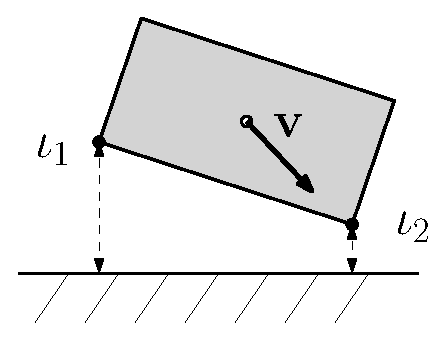
\includegraphics[width=\textwidth]{example1.eps}
\caption{$i_1,i_2\notin\Ic_{\text{c}}$}
\label{fig:3example1}
\end{subfigure}
\quad
\begin{subfigure}[b]{0.4\textwidth}  
\centering 
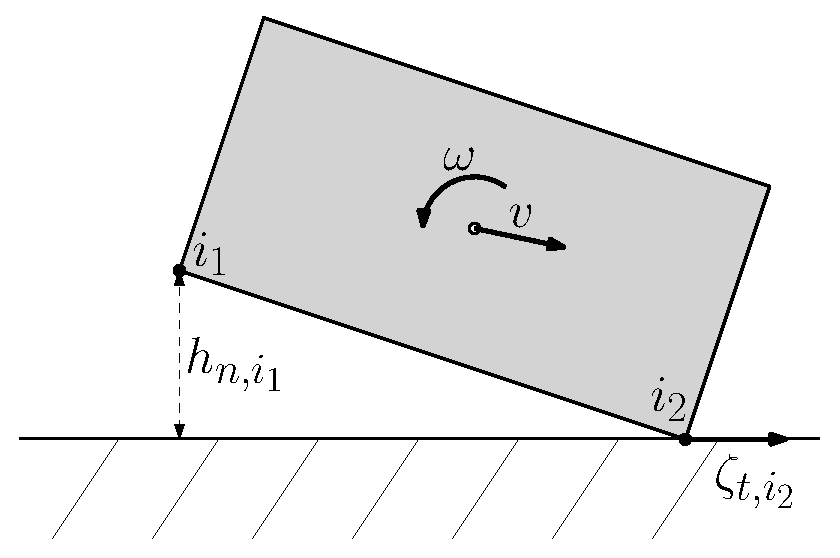
\includegraphics[width=\textwidth]{example2.eps}
\caption{$i_1\notin\Ic_{\text{c}}$, $i_2\in\Ic_{\text{sl}}$}
\label{fig:3example2}
\end{subfigure}
\vskip\baselineskip
\begin{subfigure}[b]{0.4\textwidth}   
\centering 
\includegraphics[width=\textwidth]{example3.eps}
\caption{$i_1,i_2\in\Ic_{\text{sl}}$}
\label{fig:3example3}
\end{subfigure}
\quad
\begin{subfigure}[b]{0.4\textwidth}   
\centering 
\includegraphics[width=\textwidth]{example4.eps}
\caption{$i_1,i_2\in\Ic_{\text{st}}$}
\label{fig:3example4}
\end{subfigure}
\vskip\baselineskip
\begin{subfigure}[b]{\textwidth}   
\centering 
\includegraphics[width=.8\textwidth]{exampletraj.eps}
\caption{The state trajectory of the system.}
\label{fig:3exampletraj}
\end{subfigure}
\caption{An example trajectory of a block moving towards a surface with velocity $v$. The block starts with both contact points $i_1$ and $i_2$ in open contact and through three events the block ends with both contact points in closed contact stick.} 
\label{fig:mean and std of nets}
\end{figure}

\section{First-order approximation of trajectories with ordered guard-activations}
Use Rijnen2017 alot
\begin{itemize}
\item LTTHS (Rijnen2017)
\item First-order accuracy (Rijnen2017)
\end{itemize}
\section{Stability analysis for linear time-triggered hybrid systems}

\section{Summary}


%% new chapter %%
\cleartooddpage
\chapter{Tracking for Hybrid Systems: Simultaneous State-Input-Triggered Events}\label{ch:simult}
\cite{Rijnen2018}
\section{Simultaneous guard-activation}
\begin{itemize}
\item Simultaneous events and assumptions(same post-event mode,associativity)
\item Event character, mode descriptor, micro counter, historical notation
\item Unidirectional event completion
\end{itemize}
\section{First-order approximation for trajectories with simultaneous guard-activation}
\begin{itemize}
\item Positive homogeneity
\item Positive homogeneous jump gain
\item PHTTHS (Positive homogeneous time-triggered hybrid system)
\end{itemize}

\section{Stability analysis for positively homogeneous time-triggered hybrid systems}

\section{Summary}
\end{document}